% Chapter 7

\chapter{Experiment B: Relationsvorhersage mit Wortvektorrepräsentationen} % Main chapter title

\label{Chapter7} % For referencing the chapter elsewhere, use \ref{Chapter1}

%----------------------------------------------------------------------------------------

\begin{itquote}
Q: Why did the multithreaded chicken cross the road?
A: to To other side . get the
\flushright
\textsc{Jason Whittington}
\end{itquote}

\section{Idee}

Gegeben ist ein Vektorraum $V$ mit Wortvektoren $\vec{u}, \vec{v} \in V$ und $\vec{u},\vec{v}\in\mathbb{R}^d$.
Gesucht ist eine Funktion $\phi$, die ein Vektorenpaar in einen Relationsraum abbildet: $\phi: \mathbb{R}^d \to \mathbb{R}^e$, wobei
nicht zwangsläufig $d = e$.\\
In ihrer einfachsten Form bildet sie einfach die Differenz $\vec{d}$ der beiden Vektoren:
\begin{equation}
  \phi(\vec{u}, \vec{v}) = \vec{v} - \vec{u} = \vec{d}
\end{equation}

\section{Algorithmus}

Der Grundalgorithmus (siehe Abbildung \ref{fig:algo1}) versucht nun, alle Kombinationen von Wortvektoren zu bilden und über diese
und den Differenzvektor zu bilden. Alle Kombinationen würde bei $n$ Vektoren in $n * n = n^2$ Vektoren resultieren.
Zwar ist $\phi(\vec{u}, \vec{v}) \neq \phi(\vec{v}, \vec{u})$, jedoch wäre die Berechnung beider Differenzvektoren redundant,
da sie lediglich Spiegelungen voneinander im Raum sind und so diesselbe Information enthalten. Die Berechnung
der Differenz in nur eine Richtung reduziert die Anzahl der Vektoren dadurch zu $\frac{n * (n-1)}{2}$.

\begin{figure}[h]
  \centering
  \begin{algorithm}[H]
    \KwData{Menge von Vektorpaaren $\mathcal{C}$}
    \For{$(\vec{u}, \vec{v}) \in \mathcal{C}$}{
      $\vec{d} = \vec{v} - \vec{u}$;
    }
  \end{algorithm}
  \caption[Einfacher Projektionsalgorithmus]{Einfacher Projektionsalgorithmus.\label{fig:algo1}}
\end{figure}

Gegeben einer Menge relevanter Kombinationen $\mathcal{C}$ mit Vektorpaaren gilt also:
\begin{equation}
  \forall (\vec{u}, \vec{v}) \in \mathcal{C}: (\vec{v}, \vec{u}) \notin \mathcal{C}
\end{equation}

Eine Modifikation des Algorithmus besteht daran, das Berechnen von $\vec{d}$ ab eine Bedingung zu knüpfen.
Gegeben sei eine Menge von Sätzen (ein Korpus) $\mathcal{K}$ mit $n$ Sätzen $s_i$ sodass $\mathcal{K} = \{s_i\}_{i=1}^{n}$ mit
$m$ Wörtern $w_{ij}$ pro Satz $s_i = \{w_{ij}\}_{j=1}^m$. Eine Kookkurrenz von zwei Begriffen (\emph{types}) $t_1$ und $t_2$
besteht demnach, falls im Korpus mindestens ein Satz existiert, in dem beide gleichermaßen vorkommen. Dazu können wir
eine Funktion $\Lambda$ definieren, die die Anzahl der Kookkurrenzen bestimmt:
\begin{equation}
  \Lambda(t_1, t_2) = |\{s_i | \exists w_{ij} = t_1 \land \exists w_{ij} = t_2 \land t_1\neq t_2\}_{i=1}^{n}|
\end{equation}
Eine mögliche Einschränkung besteht darin, in einem geänderten Algorithmus (siehe Abbildung \ref{fig:algo2}) das Berechnen von $\vec{d}$ nur
dann zu erlauben, wenn die Anzahl der Kookkurrenzen der zu den Vektoren $\vec{v}(t_1), \vec{v}(t_2)$ gehörenden Begriffe $t_1, t_2$
einen bestimmten Schwellenwert $\gamma$ überschreitet, also $\Lambda(t_1, t_2) > \gamma$.

\begin{figure}[h]
  \centering
  \begin{algorithm}[H]
    \KwData{Menge von Vektorpaaren $\mathcal{C}$}
    \For{$(\vec{v}(t_1), \vec{v}(t_2)) \in \mathcal{C}$}{
      \If{$\Lambda(t_1, t_2) > \gamma$}{
        $\vec{d} = \vec{v}(t_2) - \vec{v}(t_1)$;
      }
    }
  \end{algorithm}
  \caption[Modifizierter Projektionsalgorithmus]{Modifizierter Projektionsalgorithmus, bei dem die zu den Vektoren gehörigen
  Begriffe über $\gamma$ Mal im Korpus im gleichen Satz aufgetreten sein müssen, damit $\vec{d}$ errechnet wird.\label{fig:algo2}}
\end{figure}


\section{Parallelisierter Algorithmus}\label{sec:para-algo}

Doch selbst mit den erwähnten Einschränkungen skaliert dieser Algorithmus nur bedingt. Um dem entgegenzuwirken, soll nun
versucht werden, diesen mithilfe von \emph{Multithreading} zu parallelisieren. Bei dieser Technik beschäftigt ein Rechenprozess
mehrere Prozessstränge (\emph{Threads}), die miteinander kommunizieren und bei Bedarf synchronisiert werden können,
während sie Teile eines Problems lösen.\\
Ein beliebtes Muster, das Verhältis zwischen mehreren Threads zu definieren besteht im \emph{Master-Slave}-Muster.
Dabei fungiert ein Subprozess als Aufseher, der seine Arbeiterprozesse überwacht, sie mit Daten versorgt und in manchen
Fällen untereinander koordiniert.\\ \\

\begin{figure}[h]
  \centering
  \begin{algorithm}[H]
    \KwData{Menge von Vektorpaaren $\mathcal{C}$}
    \KwData{Menge von erledigten Vektorpaaren $\mathcal{C}'$ (Anfangs $\mathcal{C}' = \varnothing$)}
    \KwData{Menge von Threads $\mathcal{T}=\{th\}_i^n$}
    \BlankLine
    \textbf{Klasse} \textsc{MasterThread} \\
      data = ladeDaten();\\
      \For{$th \in \mathcal{T}$}{
        starteThread($th$, data);
      }
      \For{$th \in \mathcal{T}$}{
        beendeThread($th$);
      }

    \BlankLine
    \textbf{Klasse} \textsc{WorkerThread} \\
    \For{$(\vec{v}(t_1), \vec{v}(t_2)) \in \mathcal{C}$}{
      \If{$(\vec{v}(t_1), \vec{v}(t_2)) \notin \mathcal{C}'$}{
        \If{$\Lambda(t_1, t_2) > \gamma$}{
          $\vec{d} = \vec{v}(t_2) - \vec{v}(t_1)$;
        }
        $\mathcal{C}'$ = $\mathcal{C}' \cup (\vec{v}(t_1), \vec{v}(t_2))$;
      }
    }
  \end{algorithm}
  \caption[Parallelisierter Projektionsalgorithmus]{Parallelisierter Projektionsalgorithmus, bei dem die zu den Vektoren gehörigen
  Begriffe über $\gamma$ Mal im Korpus im gleichen Satz aufgetreten sein müssen, damit $\vec{d}$ errechnet wird. Ein Master-Thread
  verteilt zudem die Aufgaben an Worker-Threads, die diese Berechnungen übernehmen und erledigt Vektorpaare in einer Menge ablegen.
  \label{fig:algo3}}
\end{figure}

In diesem konkreten Fall ist der Master-Thread dafür verantwortlich, alle benötigten Daten in entsprechende Datenstrukturen
zu laden, sie den Worker-Threads bereitzustellen und letztere gemeinsam zu starten und zu beenden, sobald ein bestimmtes
Abschlusskriterium der Aufgabe erfüllt ist.
Zusätzlich wird eine Menge eingeführt, in die Paare von Vektoren hinzugefügt werden, sofern für sie von einem Thread
ein Differenzvektor ausgerechnet wurde (siehe Abbildung \ref{fig:algo3}). Damit nun keiner der Threads redundante Berechnungen durchführt, prüft er, ob sein
aktuelles Vektorpaar sich in dieser Menge befindet und schon abgehakt wurde\footnote{Damit dies möglichst schnell funktioniert,
wird das Vektorpaar durch eine Hashfunktion in einen Wert umgewandelt. Diese wird so gewählt,
sodass $h(\vec{v}(t_1), \vec{v}(t_2)) = h(\vec{v}(t_2), \vec{v}(t_1))$.}.\\

Als Grundlage der Daten wurde das Datenset Mark I gewählt, da es in den meisten der Evaluationsaufgaben
als bestes Abschnitt. Mit $\gamma = 100$ resultierte das Procedere in einem neuen Menge an Daten mit insgesamt
X Differenzvektoren [GENAUE ZAHL EINFÜGEN] mit einer Größe von X,X GB [GENAUE GRÖSSE EINFÜGEN].\\
Um den Gewinn durch Multithreading zu verdeutlichen, wurden darüber hinaus die Rechenzeiten gemessen (siehe Abbildung \ref{fig:times}).
Gerechnet wurde auf eine Hardware mit 40 Prozessorkernen und [RESTLICHE SPECS EINFÜGEN].

\section{Evaluation}

Die Evaluation der im vorherigen Schritt gewonnen Daten findet folgendermaßen statt: Für jedes gewonnene Cluster $c$ wird für
jedes Paar von Vektoren die Zughehörigkeit der entsprechenden Wörter zu einer \textsc{Freebase}-Relation $r$ geprüft.
Dem gesamten Cluster kann dann die Relation $r_c$ zugeordnet werden, die die meisten Treffer zu verzeichnet hat.

\begin{equation}
    r_c = \underset{r \in R}{argmax}\ \sum_{(\vec{v}(w_1), \vec{v}(w_2)) \in c}  \mathbbm{1}_{r}((w_1, w_2))
\end{equation}

Die ``Reinheit'' $P$ eines Clusters kann dann errechnet werden, indem der Anteil der zur Relation des gesamten Clusters
zugehörigen Wortpaaren bestimmt wird\footnote{Die Indikatorfuntion mit $\mathbbm{1}_{r_c}((w_1, w_2))$ liefert $1$, wenn
$(w_1, w_2) \in r_c$ gilt, ansonsten $0$.}:

\begin{equation}\label{form:purity}
    P(c) = \sum_{(\vec{v}(w_1), \vec{v}(w_2)) \in c} \mathbbm{1}_{r_c}((w_1, w_2))\ /\ |c|
\end{equation}

Diese Metrik bestraft allerdings, wenn in einem Cluster neue Paare einer Relation vorkommen, die noch nicht in \textsc{Freebase}
vorhanden sind. Da dies allerdings auch ein Teilziel dieses Ansatzes war, ebensolche Paare neu aufzufinden, wird noch
eine modifizierte Version dieser Metrik behandelt: Es gilt dabei vor allem, unbekannte richtige Wortpaare von falschen
zu unterscheiden. Zu diesem Zweck wird die Annahme getroffen, dass alle Vektoren $\vec{v}(h)$ und $\vec{v}(t)$, die zu den Kopfentitäten $H_c$ und
den Fußentitäten $T_c$ gehören, recht ähnlich sind. So wird für jedes Cluster zunächst für ebendiese Entitäten ein Durchschnitt
errechnet, deren Zugehörigkeit zu $r_c$ festgestellt wurde:

\begin{equation}
  \tilde{h} = \sum_{\vec{v}(h) \in H_c} \vec{v}(h)\ /\ |H_c|
\end{equation}

\begin{equation}
  \tilde{t} = \sum_{\vec{v}(t) \in H_c} \vec{v}(t)\ /\ |T_c|
\end{equation}

Demnach erweitern wir $r_c$ um die Wortpaare, deren Vektoren den durchschnittlichen Kopf- und Fußvektoren ähnlich genug sind.
Zu diesem Zweck wird ein Schwellenwert $\tau$ definiert, den ein potenziell zu $r_c$ zugehöriges Wortpaar im Bezug auf
Cosinusänlichkeit (siehe \ref{form:cossim}) nicht unterschreiten darf:

\begin{equation}
  r_c^+ = r_c\ \cup\ \{(w_1, w_2)| (\vec{v}(w_1), \vec{v}(w_2)) \in c\ \land\ cos(\vec{v}(w_1), \tilde{h}) \geq \tau\ \land\ cos(\vec{v}(w_2), \tilde{t}) \geq \tau\}
\end{equation}

Auf Basis der Gleichung \ref{form:purity} folgt für die modifizierte Reinheit eines Wortpaarclusters $P^+$:

\begin{equation}
  P^+(c) = \sum_{(\vec{v}(w_1), \vec{v}(w_2)) \in c} \mathbbm{1}_{r_c^+}((w_1, w_2))\ /\ |c|
\end{equation}

\section{Ergebnisse}

Vorgreifend soll angemerkt werden, dass es nicht möglich war, endgültige Ergebnisse mithilfe der vorher beschriebenen
Evaluationsmetrik $P^+(\cdot)$ zu erzeugen. Die genauen Gründe hierfür werden im nächsten Abschnitt \ref{sec:zwi-dis}
genauer beleuchtet. Dementsprechend sollen an dieser Stelle Zwischenergebnisse vorgestellt werden.\\

\begin{figure}[h]
  \centering
  \begin{multicols}{2}
    \textbf{Cluster A}\\
    $\vdots$\\
    \columnbreak
    \textbf{Cluster B}\\
    $\vdots$\\
  \end{multicols}
  \begin{multicols}{2}
    \textbf{Cluster C}\\
    $\vdots$\\
    \columnbreak
    \textbf{Cluster D}\\
    $\vdots$\\
  \end{multicols}
  \caption[Auszug aus verschiedenen Wortpaarclustern]{Auszüge aus einigen Wortpaarclustern, die mit in dem Abschnitt
  \ref{sec:para-algo} vorgestellten Ansatz erzeugt wurden.\label{fig:clusters}}
\end{figure}

Wie Abbildung \ref{fig:clusters} zu entnehmen ist, in der einige Auszüge aus Clustern beispielhaft dargestellt sind,
fällt es schwer, die dort aufgeführten Wortpaar ingesamt einer Relation zuzuordnen. Im Gegenteil gelingt dies selbst für
einzelne Paare nicht, siehe beispielweise ``Beispiel 1'' oder ``Beispiel 2''.\\
Es zeigt sich, dass auch das Kookkurrenz-Feature zu keiner Besserung der Ergebnisse geführt hat. Aufgrund der scheinbaren
Zufälligkeit der Ergebnisse erschien es auch nicht mehr sinnvoll, weitere Schritte auf Basis dieser Daten (vor allem Evaluation)
durchzuführen.\\

\section{Zwischenfazit}\label{sec:zwi-dis}

Wie der letzte Abschnitt der gezeigt hat, entsprechen die Ergebnisse nicht den vorher gefassten Hoffnungen.
Im Folgenden soll ein Versuch unternommen zu erklären, welche Probleme zu diesen Resultaten geführt haben und welche
Implikationen diese besitzen.

\subsection{Daten}\label{sec:zwi-dis-data}

Will man das Scheitern unmittelbar auf einen Faktor zurückführen, so liegen die zugrunde liegenden Daten am nächsten.
Es lassen sich im Bezug auf jene folgende Punkte feststellen:
\begin{itemize}
  \item \textbf{Menge}\\ Selbst mit dir Reduzierung der resultierenden Daten von $n^2$ auf $\frac{n*(n-1)}{2}$ ist die
  Datenmenge noch sehr groß, gerade wenn das anfänglich Wortvektorset auf einem großen Vokabular wie dem des Decow-Korpus aufbaut.
  Dies stellt hohe Anforderung an die Skalierbarkeit aller involvierter Algorithmen und fordert Einschränkungen auf verschiedener
  Ebene, wodurch mögliche spätere Entdeckung eventuell vorenthalten werden könnten.
  \item \textbf{Rauschen}\\ In den Enddaten ist der überwiegende Teil der Datenpunkte keiner sinnvollen Relation zuzuordnen.
  Dadurch verrauschen diese mögliche sinnvolle Relationscluster, die darin untergehen (vgl. Abbildung \ref{fig:proj_map}). Die resultierenden Cluster sind sehr
  schwammig, da sie sich schlecht vom Hintergrundrauschen abgrenzen. Dies ist beispielsweise durch den Wert des Silhouettenkoeffizienten\footnote{
  Der Silhoettekoeffizient $s_C$ beschreibt das durchschnittliche Verhältnis vom Abstand eines Punktes zu seinem Clusterzentrum gegnüber
  des nächsten Clusterzentrums. $-1 \leq s_C \leq 1$.}
  erkennbar, der bei den Experimenten immer kurz unter Null lag\footnote{Für ein gutes Clustering wird ein Wert von $s_C \geq 0,75$
  erwartet.}.
  \item \textbf{Ähnliche Distanzvektoren}\\
  Der beschriebene Ansatz wurde unter der Annahme verfolgt, dass für Wortpaare einer Relation $R=\{(h_j, t_j\}_{j=0}^m$
  folgendes gilt:
  \begin{equation}
    \vec{v}(t_0) - \vec{v}(h_0) \approx \vec{v}(t_1) - \vec{v}(h_1) \approx \ldots \approx \vec{v}(t_m) - \vec{v}(h_m)
  \end{equation}
  Anders ausgedrückt wurde aufgrund vorheriger Arbeiten die Hypothese aufgestellt, dass sich die Distanzvektoren von
  Wortpaaren derselben Relation ähneln. Durch die Ergebnisse wurde diese Hypothese nicht widerlegt (im Gegenteil scheinen
  andere Arbeiten wie (\cite{bordes2013translating}) oder (\cite{lin2015learning}) diese Annahmen zu bestätigen), jedoch
  gilt diese Eigenschaft nicht \textbf{exklusiv} für diese Untermenge an Vektorenpaaren.\\
  Nehmen wir beispielsweise im ursprünglichen Vektorraum mit Wortvektoren das folgende Szenario an: Wir finden dort
  zwei Cluster $C_1$ und $C_2$ vor. Die zu den Vektoren zugehörigen Cluster weisen eine semantische Ähnlichkeit auf
  und liegen deshalb nahe beieinander, z.B. Vornamen wie \emph{Julia} und \emph{Hans} in $C_1$ und Städte wie
  \emph{Barcelona} und \emph{Paris} in $C_2$. Daraus ergibt sich Folgendes:
  \begin{equation}
    \begin{split}
      \vec{v}(Julia) \approx \vec{v}(Hans) \land \vec{v}(Barcelona) \approx \vec{v}(Paris) \implies \\
      \vec{v}(Julia) - \vec{v}(Barcelona) \approx \vec{v}(Hans) - \vec{v}(Paris)
    \end{split}
  \end{equation}
  Anders ausgedrückt: Auch wenn sich semantische Information in den Wortvektoren dadurch manifestiert, dass ähnliche
  Ausdrücke in ihren Clustern nahe beinander liegen, können Distanzvektoren aus Wortenpaaren der gleichen Cluster ähnlich sein,
  ohne semantisch in irgendeinem Zusammenhang zu stehen. Dies führt schlussendlich dazu, dass die wenigen Cluster, die
  im Relationsraum gefunden werden, zwar aus Wortpaaren mit ähnlichem Differenzvektor stehen, jedoch keine ``sinnvolle''
  Relation bilden, was sicht mit dem in 6.1 eingeführtern Parameter $\gamma$ zwar verringern, allerdings nicht gänzlich
  verhindern lässt. Das Ziel, neue und legitime Relationen zu finden, wird durch diesen Trugschluss ad absurdum geführt.

\begin{figure}[h]
  \centering
  \begin{multicols}{2}
    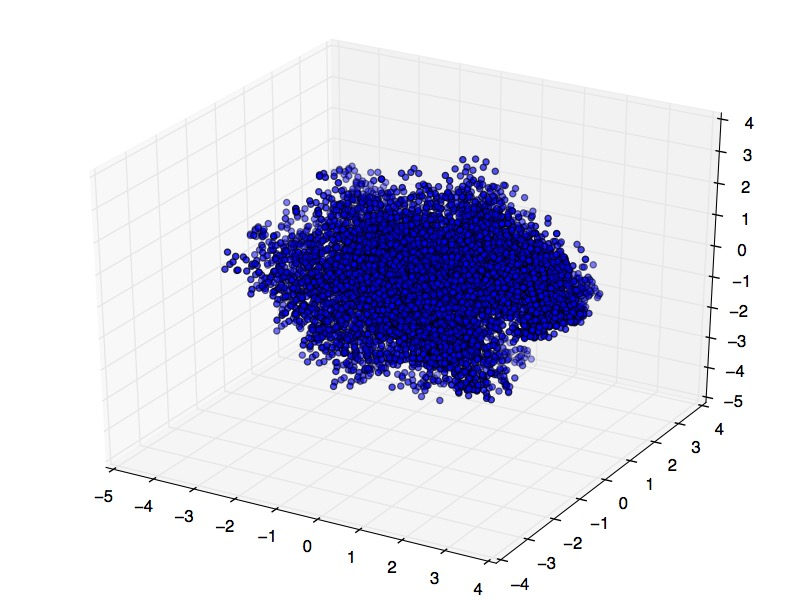
\includegraphics[width=0.5\textwidth]{../img/mappings_get10000_occ100_cos.jpg}
    \textbf{Mappings A:} $\spadesuit\clubsuit\blacksquare$
    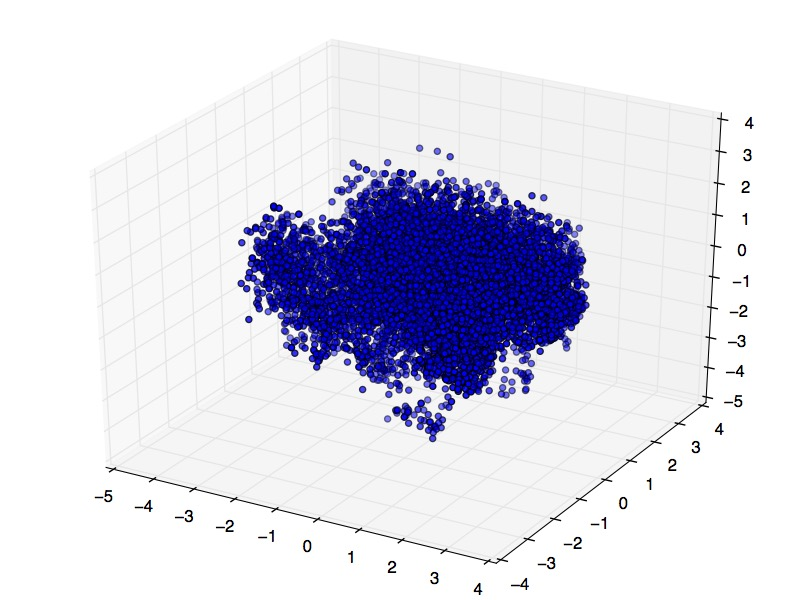
\includegraphics[width=0.5\textwidth]{../img/mappings_get10000_occ100_eucl.jpg}
    \textbf{Mappings C:} $\spadesuit\clubsuit\varheart$

    \columnbreak

    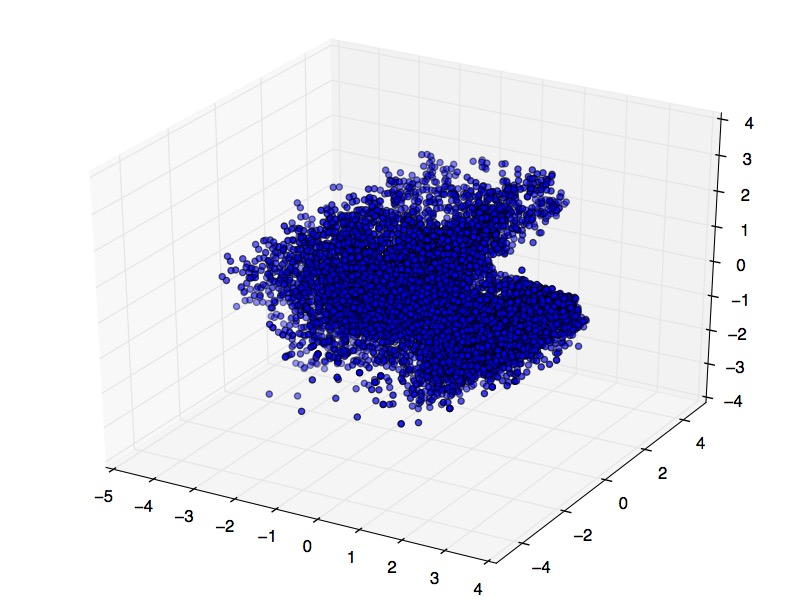
\includegraphics[width=0.5\textwidth]{../img/mappings_get10000_occ100.jpg}
    \textbf{Mappings B:} $\spadesuit\clubsuit$
    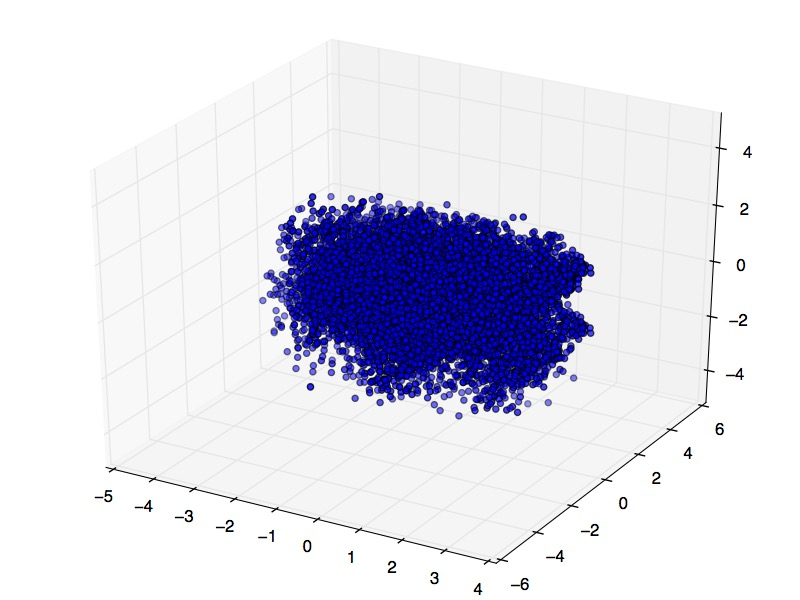
\includegraphics[width=0.5\textwidth]{../img/mappings10000_occ.jpg}
    \textbf{Mappings D:} $\spadesuit\bigstar$
  \end{multicols}

  \flushleft
  \fbox{
  \parbox{\textwidth}{
  \textbf{Feature-Legende}
  \begin{multicols}{2}
  \begin{itemize}
    \item[$\spadesuit$] $\vec{v}(t_2) - \vec{v}(t_1)$
    \item[$\bigstar$] $\Lambda(t_1, t_2) \geq 1$
    \item[$\clubsuit$] $\Lambda(t_1, t_2) \geq 100$
  \end{itemize}
  \columnbreak
  \begin{itemize}
    \item[$\blacksquare$] $cos(\vec{v}(t_2), \vec{v}(t_1))$
    \item[$\varheart$] $\parallel \vec{v}(t_2) - \vec{v}(t_1) \parallel$
  \end{itemize}
\end{multicols}
}}
  \caption[Dreidimensionale Projektionen einiger durch das Mappingverfahren resultierender Vektorräume]{Dreidimensionale
   Projektionen einiger durch das Mappingverfahren resultierender Vektorräume. Jeweils dargestellt: 10000 Vektoren.
   Symbole zeigen die jeweils genutzten Feature an. \label{fig:proj_map}}
\end{figure}

\end{itemize}

\subsection{Ansatz}

Das Fehlschlagen des Vorgehens kann auch auf einer theoretischen Ebene festgestellt werden: Das Ziel bestand darin, Wissen
über Relationen zwischen Wortpaaren zu extrahieren. Um dieses Wissen gewissermaßen ``freilegen'', muss es aber auf eine
Art und Weise innerhalb der Daten ``kodiert'' sein, wenn auch versteckt (so wie die semantische Ähnlichkeit zwischen Wörtern
durch die räumliche Nähe ihrer Vektoren und deren Dimension kodiert ist).\\
Wie beim Aufzeigen des Trugschlusses am Ende von \ref{sec:zwi-dis-data} gezeigt wurde, sind semantische Relationen nicht eindeutig
innerhalb der Daten aufzuzeigen bzw. nur dann, wenn bereits vorher bruchstückhaftes Wissen darüber vorliegt. Ohne
dieses Vorwissen sind richtige von nur scheinbaren Relationen nicht zu trennen.
